% !TeX encoding = UTF-8
% !TeX spellcheck = en_US
% !TeX root = ../main.tex
\tikzset{
	block/.style = {draw, fill=white, rectangle, minimum height=3em, minimum width=4em},
	gain/.style = {draw, fill=white, isosceles triangle, minimum height=3em, minimum width=2em},
	operator/.style= {draw, fill=white, circle},
	input/.style = {coordinate},
	output/.style= {coordinate},
	pinstyle/.style = {pin edge={to-,thin,black}},
}

\chapter{Orbit correction}
\label{sec:correction}

\section{Motivation}
The accelerators are designed so that the particles follow a given path, which is defined in the case of synchrotrons by the successive bendings involved by the magnets. As the precision of the positioning of the magnets is limited, some errors may destabilize the orbit and increase the dispersion of the particles around the theoretical orbit. In addition, the environment produces perturbations: for instance the 50~Hz of the main power, some not perfectly isolated magnetic sources.

In order not to lose electrons in the walls of the vacuum chamber but also to increase the brightness of the synchrotron radiations (and therefore to have focused electron beams), all these residual misalignment and magnetic field errors must be corrected.



\section{Monitoring and correction instruments}
To be able to correct the orbit or localize perturbations, some tools must be employed.

\subsection{Beam Position Monitors}
The position of the beam in a given direction is monitored with beam position monitors (BPM). 

Several types of BPMs exist, but the important characteristics of the one used at BESSY~II are that they provide a method
\begin{itemize}
	\item which is non invasive (it does not affect the beam or negligibly)
	\item which outputs an electric signal proportional to the distance of the beam from an arbitrary point.
\end{itemize}

This last property means that the measured value must always be subtracted by a reference value.

The raw values output by the BPMs are thus never considered and every orbit position value given (also called BPM value by misuse of language) is always, at position~$s$ and time~$t$
\begin{equation}
\Delta x_\text{BPM}(s,t) = x_\text{BPM}(s,t) - x_\text{BPM,ref}(s)
\end{equation}

\subsection{Correctors}
To correct the orbit, BESSY~II uses dipoles, also called correctors (CM) disposed around the orbit. Each dipole contributes to correcting in a given direction. 

\subsection{Monitor and corrector numbers}
The number of monitors and correctors is quite important. Because the correction method used is based on an inversion problem (see \cref{sec:response_matrix}), it is important to have an over-constrained problem. Else a perfect correction would be reached at monitor positions but unconstrained (and thus potentially arbitrary bad) elsewhere.

Therefore the number of BPMs is chosen quite greater than the number correctors.

In BESSY~II there are 
\begin{itemize}
	\item 128~BPMs, measuring both horizontal ($\text{BPM}_x$) and vertical ($\text{BPM}_x$) direction,
	\item 48~CMs for the horizontal direction ($\text{CM}_x$) and 64 for the vertical one ($\text{CM}_y$).
\end{itemize}

\section{Some documented methods}
Several global corrections methods are well documented in the literature. Local orbit bumps (presented in \cref{sec:orbit_bump}) allow local correction and are used to change the path of the orbit (during the injection time for example). The most common ones are the best corrector method and the response matrix method (see \cref{sec:most_effective_corr,sec:response_matrix}), as they provide a global correction, over the whole orbit. 

\subsection{Local orbit bumps}
\label{sec:orbit_bump}
Using local orbit bumps is a basic method that gives total control on the orbit local modification to the operator.

\subsubsection{Principle}
Adding a simple dipole on the path of a particle will focus or defocus it. As the particles must eventually return to the planned orbit, a series of dipoles can be set one after the other to design an arbitrary path. \Cref{fig:local_bump} shows a minimal example, where the black points represent the magnets. 
\begin{figure}
	\centering
	\begin{tikzpicture}[auto, node distance=1.2,>=latex']
	%\draw[help lines, yellow] (-1,-4)grid(15,3);
	% We start by placing the blocks
	\coordinate [] (lleft) {};
	\node [draw, circle, fill=black, right=2 of lleft] (leftm) {};
	\node [draw, circle, fill=black, above right=2 and 2.5 of leftm] (topm) {};
	\node [draw, circle, fill=black, right=5 of leftm] (rightm) {};
	\coordinate [right=2 of rightm] (rright) {};
	% Once the nodes are placed, connecting them is easy. 
	\draw [-] (lleft) -- node {}(leftm);
	\draw [-] (leftm) -- node {}(topm);
	\draw [-] (topm) -- node {}(rightm);
	\draw [-] (rightm) -- node {}(rright);
	\end{tikzpicture}
	\caption{\label{fig:local_bump}Local bump with 3 magnets}
\end{figure}
\todo[inline]{see Wille p127 and p286}


\subsubsection{In practice}
This solution is used for instance to shift a part of the orbit during particle injections, in order to prevent collisions. This can also be used to counter a known localized perturbation which source cannot be removed.

It is indeed very efficient to locally shift the orbit. However it cannot be used for correction, as it modify the path of the orbit itself, introducing maybe other perturbations.

\subsection{Most effective corrector method}
\label{sec:most_effective_corr}
This method is based on the fact that orbit shifts are often caused by strong localized disturbances. Its goal is to correct particularly each disturbance.

\subsubsection{Principle}
Given a distorted orbit, the optimal gain for each corrector is calculated by a mean square error algorithm (see \cref{eq:gain_bestcorr} and \cite{book:wille}). The corrector which provides the best correction is selected: it is the most effective corrector.

Let's assume that the $i$th corrector, at position $s_i$, has the optical parameters $\beta_i$, $\alpha_i$ and $\Psi_i$, and that $m$ monitors are set around the orbit with parameters $\beta_j$, $\alpha_j$ and $\Psi_j$, and read a displacement $u_j$ from the reference orbit ($1 \leq j \leq m$).

The strength $\kappa_i$ of the field at the position $s_i$ is obtained minimizing the function
\begin{equation}
	\label{eq:gain_bestcorr}
    f_i(\kappa_i) = \sum\limits_{j=1}^{m} (u_j-x_{ij}(\kappa_i))^2 
                  = \sum\limits_{j=1}^{m} (u_j- \kappa_i h_{ij})^2
\end{equation}

with, if $\Delta \Psi_{ij} := \Psi_j-\Psi_i$,

\begin{align}
    \label{eq:hij}
    x_{ij}(\kappa_i) &= \kappa_i h_{ij} \nonumber\\
                     &= \kappa_i \frac{\sqrt{\beta_i \beta_j}}{2}
                         \left[
                             \frac{\cos(\Delta \Psi_{ij}) - 2\alpha_i \sin(\Delta\Psi_{ij})}
                                  {\tan (\pi Q)} + \sin (\Delta\Psi_{ij})
                         \right].
\end{align}

It follows that 
\begin{equation}
    \kappa_i = \frac{\sum\limits_{j=1}^m u_j h_{ij}}{\sum\limits_{j=1}^m h_{ij}^2}
\end{equation}

The $i$th corrector is attributed the gain $-\kappa_i$ to compensate the field.

\subsubsection{Iterative version}
When the most effective corrector is found, the process is reiterated on the corrected orbit with the remaining correctors. By doing this until all corrector are used (or that adding a correction does not improve the orbit) a comprehensive correction is reached.

\subsubsection{Practical issue}
The problem of this method is that each corrector must be tested once, and this for each iteration: the initialization of the correction is long and is then fixed. Moreover, the correction is less efficient than the other ones presented here~\cite{book:wille}.

\subsection{Inversion of the response matrix}
\label{sec:response_matrix}
This section is mainly based on~\cite{book:wille}, \cite{art:decker-1991} and \cite{art:plouviez-1999}.

\subsubsection{Inverse problem}
This correction is based on solving the following inverse problem: the expected orbit being known, how to set the correctors in order to achieve it? To solve it, the response matrix $\mat{S}$ is introduced.

The response matrix $\mat{S}$ is defined by the equation $\vec{X} = \mat{S}\, \vec{\Theta}$ where $\vec{\Theta}$ is the \emph{kick vector} (i.e. the vector of strength of the field generated by each corrector) and $\vec{X}$ the vector of \emph{orbit change}. If the accelerator has $M$ monitors and $N$ correctors, then $\mat{S}$ is a $M \times N$ matrix. $\mat{S}$ is often termed \emph{forward} or \emph{observation matrix} because it describes the effects of a given phenomenon. Indeed, each coefficient $S_{ij}$ of the matrix is the orbit change at the position $s_i$ (of the $i$th monitor), for a kick of unity 1 at the position $s_j$ (of the $j$th corrector).

Inversing the response matrix will provide the correction to apply. Since it's very common to have more monitors than correctors, the matrix is not square. A \emph{singular value decomposition} (SVD) is used on the matrix to provide a pseudo-inversion $\mat{S}^*$ of $\mat{S}$.

Using the SVD also allows to use only the most significant singular values in the correction. This prevents to over-correct the orbit, by not considering less significant values that can result of noise in the monitors during the measure, or numerical artifacts for instance.

The correction can then be performed
\begin{equation}
\vec{\Theta} = \mat{S}^* \vec{X}.
\end{equation}

\subsubsection{Acquisition of the response matrix}
Before solving the inverse problem, the response matrix must first be determined. This can be achieved in two different ways: by describing the magnet structure and explicitly calculating the matrix or by acquiring it in an experimental way.

\paragraph{Calculation of the response matrix}
The matrix can be theoretically calculated by using the accelerator model and physics. This was already used in \cref{sec:most_effective_corr} and using the same calculations leads to setting, for the $i$th monitor and $j$th corrector,
\begin{equation}
S_{ij} = h_{ij}
\end{equation}
with $h_{ij}$ as defined in \cref{eq:hij}.

The main flaw of this method is that it is only a model which hence may not exactly represent the reality. Some misalignments of magnets or external magnetic perturbations would not be taken in account. It's however a good first approach.

\paragraph{Experimental acquisition of the response matrix}
A more common and precise way of constructing the response matrix is empirical: it suffices to give a unitary value to a corrector and to read the monitors to obtain a column $\mat{S}$. Doing so for each corrector provides the whole matrix.


\section{State of the art at BESSY II}
\label{sec:correction_state_of_art}
\subsection{The correction}
BESSY II currently uses a Fast Orbit Feedback (FOFB) which is based on a PID correction\todo{why do we need a PID?} (proportional response with gain P, integral response with gain I and derivative response with gain D) and the response matrix inversion. The full process goes as presented in \cref{fig:block_correction}.

\begin{figure}
    \centering
    \begin{tikzpicture}[auto, node distance=1.2,>=latex']
    %\draw[help lines, yellow] (-1,-4)grid(15,3);
        % We start by placing the blocks
        \node [operator] (sum) {$+$};
        \node [input, above=2 of sum.center] (xref) {};
        \node [operator, right=of sum] (prod) {$\times$};
        \node [input, above=2 of prod.center] (invS) {};
        \node [gain, right=0.7 of prod] (gain) {$\vec{W}$};
        \node [block, right=of gain] (PID) {~PID~~};
        \node [input, above=2 of PID.center] (pidcoef) {};
        \node [operator, right= of PID] (sum2) {$+$};
        \node [block, above right= 0.8 and 0.65 of sum2.center] (delay) {Delay T};
        \coordinate [right=3 of sum2.center] (straight) {};
        \node [draw, ellipse, minimum height=1.7cm, minimum width=5.5cm, below=1 of straight] (ring) {Storage Ring};
        \node [draw, ellipse, line width=1pt, dotted, minimum height=.5cm, minimum width=.8cm, above=-.25 of ring.north, label=above right:\footnotesize Correctors] () {};
        \node [draw, ellipse, line width=1pt, dotted, minimum height=.5cm, minimum width=.8cm, above=-.25 of ring.west, label=above left:\footnotesize BPMs] (BPM) {};
        \coordinate [left=1 of sum.center](leftback) {};
        
        % Once the nodes are placed, connecting them is easy. 
        \draw [->] (xref)     -- node [pos=0.85, left]{$-$} node {$\vec{X}_\text{ref}$}(sum);
        \draw [->] (sum)      -- node {$\Delta\vec{X}$} (prod);
        \draw [->] (invS)     -- node {$\mat{S}^*$}        (prod);
        \draw [->] (prod)     -- node {}             (gain);              
        \draw [->] (gain)     -- node {$\Delta\vec{\Theta}_\text{t}$}             (PID);
        \draw [->] (PID)      -- node {$\Delta\vec{\Theta}$}             (sum2);
        \draw [->] (pidcoef)  -- node[pos=0.70, above, fill=white] {PID coeff.} (PID);
        \draw [-]  (sum2)     -- node {}  (straight);
        \draw [->] (straight) |- node[pos=0, right] {$\vec{\Theta}_{(n)}$} (delay);
        \draw [->] (delay)    -| node[pos=0.92, left] {$-$} node[above] {$\vec{\Theta}_{(n-1)}$} (sum2);
        \draw [->] (straight) -- node[pos=0.80] {}  (ring);


        \draw [-]  (ring)     -| node {}             (leftback);
        \draw [->] (leftback) |- node[pos=0.5] {$\vec{X} $}  (sum.west);
\end{tikzpicture}
    \caption{\label{fig:block_correction}The correction process}
\end{figure}

The control value at round $n$ is the differential orbit 
\begin{equation}
 \Delta \vec{X}(n) := \vec{X}(n)-\vec{X}_\text{ref}
\end{equation}
which is expected to be 0. The correction provided by the weighted response matrix is then processed
\begin{equation}
\Delta \vec{\Theta}_\text{t}(n) :=  \left[ \mat{S}^{-1} \cdot \Delta \vec{X}(n) \right] \odot \vec{W}
\end{equation}
(with $\odot$ the point-wise multiplication and $\vec{W}$ the vector of weights) and modulated by the PID correction. The ideal PID has the form
\begin{equation}
H_{PID}(s) = K_p + \frac{K_i}{s} + K_d \cdot s 
\end{equation}
or, with the z transform (calculated with Euler's method),
\begin{equation}
H_{PID}(z) = K_p + \frac{K_i}{1-z} + K_d \cdot (1-z)
\end{equation}
which yields
\begin{equation}
\Delta \vec{\Theta}(n) =  K_p \cdot \Delta \vec{\Theta}_\text{t}(n) + K_i \cdot \sum\limits_{k=0}^{n-1}\Delta \vec{\Theta}_\text{t}(k) + K_d \cdot \left[\Delta \vec{\Theta}_\text{t}(n) - \Delta \vec{\Theta}_\text{t}(n-1)\right].
\end{equation}

The real correction is eventually the accumulation of all corrections
\begin{equation}
\vec{\Theta}(n) = \vec{\Theta}(n-1) - \Delta \vec{\Theta}(n).
\end{equation}

\remark The PID gains is not exactly as presented here: to prevent a too violent correction that might destabilize the current in the ring, the proportional gain is increased every correction round by 1\% until it reaches its nominal value.

\subsection{Technical overview}

The correction is naturally automatized. Because the read/write actions should be really fast, a specific infrastructure was designed. This is represented on \cref{fig:cbox_mbox}. 

\begin{figure}[!h]
    \centering
    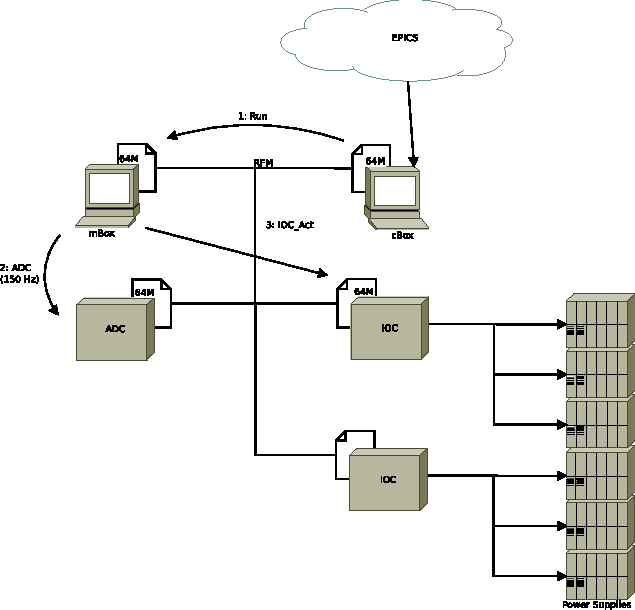
\includegraphics[width=.85\linewidth]{img/mBox_cBox}
    \caption{\label{fig:cbox_mbox}cBox and mBox: the correction infrastructure in BESSY II}
\end{figure}

All elements are connected to a reflective memory (RFM), which provides a high speed and low latency interface. This memory space is split in specified divisions to prevent data collisions.

Two main processes are operating:
\begin{itemize}
    \item the \textbf{cBox} which controls (= \textit{c}) the correction. It defines when to read the values of the BPMs and when to write the new correction values, it provides initializations values. The operators are communicating with this process to configure the correction.
    \item the \textbf{mBox} which does the math (= \textit{m}) of the correction. When allowed by the cBox, it reads the BPMs values, do the maths to define the new correction values and write them to the communication bus. This process also publish the values it reads and write so that client programs can subscribe to this data stream and reuse the values internally.
\end{itemize}

After having received the command to run from the cBox, the mBox queries the ADC (Analog-to-Digital Converter) to provide the BPM values in the RFM. The correction is then calculated (in Amperes) and the values are converted in a format easily transmissible. This data is written back to RFM and read by the IOCs (Input-Output Controllers) that relay to the power supplies alimenting the corrector magnets.

The full process is repeated at a frequency of 150~Hz. 

\section{Improvement of the correction of harmonic perturbations}
\subsection{Acquisition of the frequency-dependent response matrix}
\subsection{Correction of harmonic perturbations}
